\documentclass[twocolumn,prb,showpacs,superscriptaddress]{revtex4}
\usepackage{graphicx}

%
% warning: if you redefine \r you will have troubles with the angstrom,
% which is internally defined as \r{A}
%

\def\w{\omega}
\def\>{\rangle}
\def\<{\langle}
\def\H{\hat{H}}
\def\E{\varepsilon}
\def\vp{{v^\prime}}
\def\q{{\bf q}}
\def\G{{\bf G}}
\def\Gp{{\bf G^\prime}}
\def\rt{\tilde{r}}
\def\pt{\tilde{p}}

% -------
\usepackage{soul}
\usepackage{color}
\definecolor{yellow}{rgb}{1,1,0}
\definecolor{lightblue}{rgb}{0.6,0.6,0.9}
\sethlcolor{yellow}
% -------

\begin{document}

\title{GW method using density-functional perturbation theory}

\author{Feliciano Giustino}
\email{feliciano.giustino@materials.ox.ac.uk}
\affiliation{Department of Materials, University of Oxford, Parks Road, Oxford OX1 3PH, United Kingdom}
\affiliation{Department of Physics, University of California at Berkeley, 
Berkeley, California 94720, USA,
and Materials Sciences Division, Lawrence Berkeley National Laboratory, 
Berkeley, California 94720, USA}
\author{Marvin L. Cohen}
\author{Steven G. Louie}
\affiliation{Department of Physics, University of California at Berkeley, 
Berkeley, California 94720, USA,
and Materials Sciences Division, Lawrence Berkeley National Laboratory, 
Berkeley, California 94720, USA}
\date{\today}

\begin{abstract}
We propose a new approach to quasiparticle GW calculations based on the
direct evaluation of the Green's function and of the screened Coulomb interaction.
The Green's function is computed by using Haydock's recursion method,
and the screened Coulomb interaction is computed by using density-functional
perturbation theory. The frequency-dependent screened Coulomb interaction 
is explicitely calculated along the imaginary axis and analytically continued 
to the real axis using Pad\'e functions. We implemented the
proposed method within the empirical pseudopotential formalism and 
we studied silicon as a test case. We compare our new method with existing
approaches and illustrate our future development plans.
\end{abstract}

\pacs{71.15.-m, % Methods of electronic structure calculations
      71.15.Qe} % Excited states: methodology

\maketitle

\section{Introduction}

Importance of GW calculations, Motivation, History of the idea,
Explanation of where we are and how the manuscript is organized.

\section{Methodology overview}

\section{Green's function}

\section{Screened Coulomb interaction}

\begin{equation}\label{eq.linsys.1}
(H - \epsilon -\w) \Delta\psi = \Delta V \psi
\end{equation}
\begin{equation}\label{eq.linsys.2}
(H - \epsilon +\w) \Delta\psi = \Delta V \psi
\end{equation}

\section{Implementation}

The approach described above is currently implemented in the empirical
pseudopotential code {\tt OxfordGW} or {\tt GWdfpt}. 

\section{Results}

\section{Conclusions and outlook}

\begin{acknowledgments}
Computational resources were provided by the Oxford Supercomputing Centre.
This work was partly supported by the National Science Foundation Grant No. DMR04-39768 and by
the Director, Office of Science, Office of Basic Energy Sciences, Materials Sciences
and Engineering Division, U.\ S.\ Department of Energy under Contract No. DE-AC02-05CH11231.
\end{acknowledgments}

\appendix

\section{All frequencies in one shot}

Need to discuss pro and cons. In principle it is interesting (I tested it and it works).
The limitations: 1) cannot do selfconsistency (or can do but only one scf iteration),
hence we have to do matrix inversion for every frequency.
THIS MATRIX INVERSION IS EXPENSIVE OR NOT??
In terms of scaling it seems that mat inversion is N3 while my scf is N4...
The problem with the one-shot is that we cannot use the preconditioner,
therefore we may need many iterations for a system with a large cutoff
(say 300 iterations). 300 its / 10 frequencies = 30 -> if we can do the
scf in 3 steps (in average over the frequencies) at 20 it/scf -> 60 steps
and we are only a factor 2 above.
In cases where we need a shitload of frequencies (>100) it could be
more convenient to go through the inversion.
So probably 10 freqs scf is ok, more than 10 is not.
Also: for large systems we need large memory requirements - unless we do parallel inversion -
while the scf procedure only requires a small memory (store the deltapsi).

NOTE THAT I DID NOT WANT TO DO THE MANUAL INVERSION BECAUSE THAT
WAS THE PROCEDURE ADOPTED BY REINING LONG TIME AGO.


\section{Scaling properties}

To compare scaling of HL86 and GWHS is better to state from the start that
we consider only w=0.

\section{Condition number of the linear system}

The iterative calculation of the screened Coulomb interaction at finite real
frequencies $\w$ can be considerably more time-consuming than in the static
($\w=0$) case. Simple tests indicate that the computational effort, as given
by the number of iterations required to reach convergence, increases with 
increasing frequency $\w$. This behavior suggests that the linear system 
on the lhs of Eq.\ (\ref{eq.linsys.1}) becomes progressively more ill-conditioned 
as the frequency $\w$ increases.

In order to rationalize this observation, in the following we examine
the condition number of the linear system in Eq.\ (\ref{eq.linsys.1}).
The minimum number of iterations $N_{\rm min}$ required for the solution of
a real-symmetric problem using the conjugate gradients algorithm is given by
  \begin{equation}\label{eq.cg}
  N_{\rm min} = \frac{1}{2}\sqrt{\kappa} \log(2/\epsilon),
  \end{equation}
$\kappa$ being the condition number of the linear operator and $\epsilon$ the
target (relative) accuracy.\cite{painless.cg} In our calculations we used the 
complex biorthogonal conjugate gradient method of Ref.\ \onlinecite{jacobs} 
({\tt comp-BiCG}), which is an extension of the standard CG algorithm to the 
case of general complex matrices. While the estimate Eq.\ (\ref{eq.cg}) strictly 
holds only for the original CG algorithm, we found empirically that it also 
provides an accurate description of the convergence rate for the {\tt comp-BiCG} 
algorithm.

The condition number of a linear operator can be obtained by taking the ratio 
of its largest and smallest eigenvalues, $\kappa=|A_{\rm max}/A_{\rm min}|$.
Now, if we formally expand the one-particle Hamiltonian in terms of its valence 
$|v\>$ and conduction $|c\>$ eigenstates with eigenvalues $\E_v$ and $\E_c$, we obtain
$\H = \sum_v \E_v |v\>\<v| + \sum_c \E_c |c\>\<c|$. For a given valence state 
$|v^\prime\>$ the linear operator $\hat{A}_\vp (\w) = \H - \E_\vp + \alpha \hat{P}_v - w$ 
on the lhs of Eq.\ (\ref{eq.linsys.1}) reads
  \begin{equation}
  \hat{A}_\vp (\w)  = 
  \sum_v ( \E_v - \E_\vp + \alpha - w ) |v\>\<v| 
  + \sum_c ( \E_c - \E_\vp - w ) |c\>\<c|,
  \end{equation}
and its eigenvalues are given by $A_v = \E_v - \E_\vp + \alpha - w$ and
$A_c = \E_c - \E_\vp - w$. 

Let consider first the simplest case where $\w=0$ and $\alpha>0$. In this case 
we find by inspection that the smallest eigenvalue is $|A_{\rm min}|= \min(E_{\rm g}, |\alpha-W_{\rm occ}|)$, 
$E_{\rm g}$ being the fundamental gap and $W_{\rm occ}$ the valence bandwidth.
It is common practice to set $\alpha=2W_{\rm occ}$ in order to avoid null eigenvalues.
\cite{baroni.rmp} With this choice the smallest eigenvalue becomes $|A_{\rm min}|=E_{\rm g}$.
On the other hand, the maximum eigenvalue can be approximated by the
cutoff energy of the wavefunction basis set $|A_{\rm max}|=E_{\rm cut}$.
The cutoff energy corresponds to the largest expectation value of the Hamiltonian 
across the basis set.
In this case the condition number reads therefore $\kappa = E_{\rm cut}/E_{\rm g}$.
As an example, if we are using a planewaves cutoff of 50 Ry, the electron energy
gap is 1 eV, and the target accuracy is $\epsilon=10^{-10}$, then according to
Eq.\ (\ref{eq.cg}) the minimum number of CG iterations required to solve 
the linear system would be $N_{\rm min} = 310$. Empirical tests show that this 
estimate is indeed quite accurate.
In order to improve the convergence rate it is common to resort to preconditioning
techniques. We adopted the Teter-Payne-Allan preconditioner\cite{tpa}
in order to modify the eigenvale spectrum of the preconditioned system
and reduce the condition number to $\kappa_{\rm pc} \sim \kappa / E_{\rm cut} \sim 1-10$.
The use of the Teter-Payne-Allan preconditioner therefore should reduce the optimal 
number of iterations (for $\epsilon=10^{-10}$) down to at best $N_{\rm min,pc} = 12$. 
We confirmed this point by performing some simple tests.

We now consider the case of $\w<0$. Simple algebra shows that in this case
(ignoring preconditioning for simplicity) $\kappa = E_{\rm cut}/(E_{\rm g} + w)$
when $\alpha = 2W_{\rm occ}$. Hence in this case the larger the frequency $\w$,
the better conditioned the linear system. We verified that this is indeed the
case by direct calculation.

The worst case in terms of condition number is found when $\w>0$. 
In fact, as soon as $\w>E_{\rm g}$, the linear operator acquires null eigenvalues 
corresponding to the resonance condition $w = \E_c - \E_\vp$. The associated condition
number $\kappa(\w)$ exhibits significant structure, reflecting
the joint density of states of the system. Even after preconditioning the system, 
the number of iterations required to achieve convergence can be as high as 
$N_{\rm min} = 500$, thus rendering this avenue unpractical.
The calculation of the screened Coulomb interaction for frequencies slightly
off the real axis $\w+i\eta$, with $\w>0$ and small $\eta$, leads only to a negligible
improvement of the convergence rate.
Furthermore, the difficulty in finding the solution of the linear system 
for large positive frequencies is accompanied by the additional difficulty 
in obtaining a proper sampling of the Brillouin zone in order to correctly 
describe the pole $w = \E_c - \E_\vp$.

Alltogether, these considerations suggest that an iterative solution of the
linear system along the real axis is not convenient from the computational
viewpoint. For this reason we decided to perform the calculation of $W_{\G,\Gp}(\q,\w)$
along the imaginary axis and then to analitically continue the functions
to the real axis using a Pad\'e approximant.\cite{pade1,pade2,pade3}

The motivation behind our choice is easily understood by considering a simple
plasmon-pole model of the screened Coulomb interaction:\cite{hl86}
  \begin{equation}
  W(\w) = v + (W_0 -v) \Big( \frac{w_{\rm p}/2}{w+w_{\rm p}} - \frac{w_{\rm p}/2}{w-w_{\rm p}} \Big),
  \end{equation}
$\w_{\rm p}$ being the pole energy and $W_0$ the static screened Coulomb interation.
Analytical continuation of this function to the imaginary axis (with $\w=i\beta$ and $\beta$ real)
yields
  \begin{equation} \label{eq.pp.im}
  W(\w=i\beta) = v + (W_0 -v) \frac{1}{1+(\beta/w_{\rm p})^2}.
  \end{equation}
Hence, the screened Coulomb interaction along the imaginary axis contains the same
amount of information as the one on the real axis ($w_{\rm p}$ and $W_0$), and 
in addition has no singularities and is extremely smooth.
In particular, for $\w=i\beta$ (assuming no preconditioning
and $\alpha=0$ for simplicity) the condition number reads 
$\kappa=[(E_{\rm g}^2+\beta^2)/(E_{\rm cut}^2+\beta^2)]^\frac{1}{2}$,
which clearly tends to unity at large $\beta$.

In summary, by solving iteratively the linear system along the imaginary
axis we circumvent the difficulties related to the large condition numbers and 
dense Brillouin zone sampling occurring at real frequencies. Within the present
approach, the worst case scenario for the solution of the linear system 
corresponds to the static case $W_{\G,\Gp}(\q,\w=0)$.

\section{Preconditioned complex biconjugate gradient algorithm}

In this section we illustrate our implementation of the preconditioned 
{\tt comp-BiCG} algorithm. The original algorithm of Ref.\ \onlinecite{jacobs}
was introduced without preconditioning. We applied the preconditioning
by following the general recipie of Ref.\ \onlinecite{painless.cg}.

We are interested in solving the linear system
  \begin{equation}\label{eq.axeqb}
  Ax=b,
  \end{equation}
with A a complex linear operator (not necessarily Hermitian), $b$ a complex 
vector, and $x$ the solution vector.
The {\tt comp-BiCG} algorithm is an extension of the standard conjugate
gradients method which generates two sequences of residuals in such a
way that successive residuals $r_n$ and $\rt_{n+1}$ are biorthogonal.\cite{jacobs}
The algorithm starts by setting the initial residuals
$r_0 = b-Ax_0$ and $\rt_0=r_0^\star$, and the initial search directions to 
$p_0=r_0$ and $\pt_0=p_0^\star$.
Subsequently, for each iteration $n=0,1,\cdots,N-1$ we update the solution
vector, the search directions, and the residuals as follows:
  \begin{eqnarray}
  \alpha_n & = & \<\rt_n|r_n\>/\<\pt_n|Ap_n\> \nonumber \\ \nonumber
  x_{n+1} & = & x_n + \alpha_n p_n \\ \nonumber
  r_{n+1} & = & r_n - \alpha_n Ap_n \\ \nonumber
  \rt_{n+1} & = & \rt_n - \alpha_n^\star A^\dagger \pt_n \\ \nonumber
  \beta_n & = & - \<A^\dagger\pt_n|r_{n+1}\>/\<\pt_n|Ap_n\> \\ \nonumber
  p_{n+1} & = & r_{n+1} + \beta_n p_n \\ \nonumber
  \pt_{n+1} & = & \rt_{n+1} + \beta_n^\star \pt_n. \\ \nonumber
  \end{eqnarray}
The time-consuming step in this algorithm is the application of the operator 
$A$ to the search directions $p_n$ and $\pt_n$. There are two such operations 
per iteration, therefore the computational complexity is twice that of the
standard conjugate gradient algorithm (where there is only one such operation
per iteration).

Preconditioning is achieved by left-multiplying the linear system in Eq.\ (\ref{eq.axeqb}) 
by $M^{-1}$ ($M^{-1}Ax=M^{-1}b$). If we assume that the preconditioner $M$ can be 
written as $M=E^{\rm T}E$, then we can rewrite the system as follows:
  \begin{equation}
  E^{-1}AE^{-{\rm T}} E^{\rm T}x = E^{-1}b.
  \end{equation}
By defining $A^\prime=E^{-1}AE^{-{\rm T}}$, $x^\prime=E^{\rm T}x$, and $b^\prime=E^{-1}b$
we obtain the transformed system $A^\prime x^\prime=b^\prime$, for which the
standard {\tt comp-BiCG} method applies.
While this procedure is formally advantageous, it is not convenient to explicitely
manipulate the linear operator (which in our case is actually unknown), and it is
convenient to perform a few transformations to rewrite the procedure in terms of
$A$, $b$, and $x$. For this purpose we make the following substitutions:
$r^\prime = E^{-1}r$, $p^\prime=E^{\rm T} p$. Some algebra leads straightforwardly
to the preconditioned version of the {\tt comp-BiCG} algorithm:
  \begin{eqnarray}
  \alpha_n & = & \<\rt_n|M^{-1}r_n\>/\<\pt_n|Ap_n\> \nonumber \\ \nonumber
  x_{n+1} & = & x_n + \alpha_n p_n \\ \nonumber
  r_{n+1} & = & r_n - \alpha_n Ap_n \\ \nonumber
  \rt_{n+1} & = & \rt_n - \alpha_n^\star A^\dagger \pt_n \\ \nonumber
  \beta_n & = & - \<A^\dagger\pt_n|M^{-1}r_{n+1}\>/\<\pt_n|Ap_n\> \\ \nonumber
  p_{n+1} & = & M^{-1}r_{n+1} + \beta_n p_n \\ \nonumber
  \pt_{n+1} & = & M^{-1}\rt_{n+1} + \beta_n^\star \pt_n, \\ \nonumber
  \end{eqnarray}
with the initializations: $r_0=b-Ax_0$, $p_0=M^{-1}r_0$, $\rt_0=r_0^\star$,
$\pt_0=p_0^\star$.
The additional cost associated with the use of the preconditioner is negligible
with respect to the overall cost of the {\tt comp-BiCG} method.
In this work we successfully have used the algorithm derived above by adopting the
Teter-Payne-Allan preconditioner.\cite{tpa}

\section{Analytical continuation using Pad\'e approximants}

In order to perform the analytic continuation of the screened Coulomb interaction
from the imaginary frequency axis to the real axis, we employ diagonal Pad\'e 
approximants.\cite{pade1,pade2,pade3}
A Pad\'e approximant of order $N$ is a rational function which matches exactly the fitted function
in $N$ distinct points. For instance, in the case of odd $N$, the Pad\'e approximant
reads
  \begin{equation}
  P_N(x) = \frac{p_0+p_1x+p_2x^2+\cdots+p_{(N-1)/2}x^{(N-1)/2}}{1+q_1x+q_2x^2+\cdots+q_{(N-1)/2}x^{(N-1)/2}},
  \end{equation}
where the coefficients have to be determined in such a way that $P_N(x_n)=f(x_n)$ for $n=1,\cdots,N$
if $f(x)$ is the target function.
Empirical tests show that, in order to reproduce correctly the main features in the 
frequency dependence of the screened Coulomb interaction, the order of the approximant
must be at least $N\ge5$.
This observation can be rationalized by looking once more at the simple plasmon-pole
model given by Eq.\ (\ref{eq.pp.im}). From this expression is clear that the gross
features of the functions are defined once we fix the following parameters:
(i) the value at $w=0$; (ii) the asymptotic value of 1; (iii) the asymptotic derivative
going to zero; (iv) the flat slope at $w=0$; (v) the half-width at half maximum.
In practice a Pad\'e approximant with fewer than $N=5$ points will not in general
be able to capture the plasmon-pole structure of $W(\w)$.
Although this appear as a limitation, we recongnize that 3 out of the 5 constraints
needed to reproduce the plasmon pole approximation can be imposed without performing
any calculations. There remains two points to be calculated, which is the same
amount of information needed for the PP approximation.

It remains to investigate the possibility of a multipole expansion as suggested
by Godby and Needs. This latter seems a more natural choice, since it enforces
from the outset the functional shape of the dielectric function.
However, after some experimentation (we used the simplex downhill method of 
Nelder and Mead as implemented in the NAG library) we have found that the nonlinear 
optimization problem associated with the search of the energy, strengths, and widths of the
plasmon-like poles is extremely sensitive to the choice of the initial guess.
Therefore, while a multipole expansion may represent an advantageous choice
for simple cases where some information about the system is available,
it does not seem appropriate for an automatic procedure where the analytic
continuation is performed for every $\G$, $\Gp$, and $\q$ of the screened
Coulomb interaction without manual intervention.
The Pad\'e approximants appear much more robust in this respect, and a few
imaginary frequencies are sufficient to reproduce the plasmon-pole structure
along the real axis, together with information on the pole width.
Our investigation supports the view already expressed in Ref.\ \onlinecite{pade3}.

\begin  {figure}
\begin  {center}
%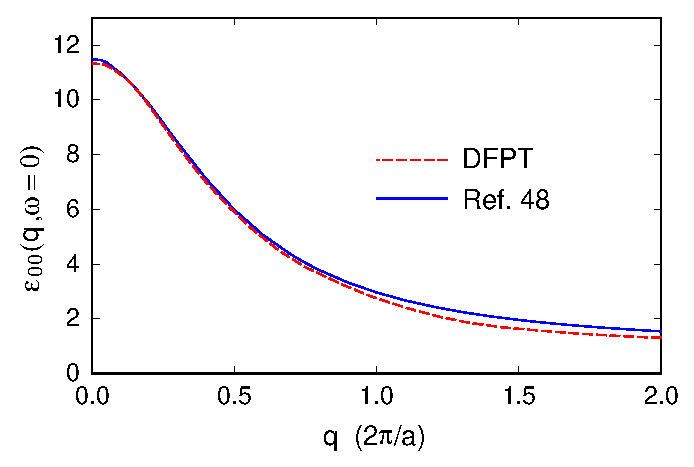
\includegraphics[width=7.5cm]{fig1.eps}
\end    {center}
\caption{\label{fig1}
        Comparison of the dielectric function calculated for silicon 
        on the real axis and the analytically continued function starting
        from imaginary frequencies. The three panels correspond to the
        cases illustrated in Fig.\ 3 of Ref.\ \onlinecite{hl86}.
        }
\end    {figure}


\begin{thebibliography}{99}

\bibitem{hl}
L. Hedin and S. Lundqvist,
Effects of the electron-electron and the electron-phonon interaction in
the one-electron states of solids,
in {\it Solid State Physics}, ed. by F. Seitz, D. Turnbull, and
H. Ehrenreich, (Academic, New York, 1969), vol.\ 23, pag. 1.

\bibitem{hl86}
M. Hybertsen and S. G. Louie, 
Phys.\ Rev.\ B {\bf 34}, 5390 (1986).

\bibitem{painless.cg}
G.\ H.\ Golub and C.\ F.\ Van Loan, {\it Matrix Computations} (John Hopkins University Press, Baltimore, 1983).

\bibitem{jacobs}
D.\ A.\ H.\ Jacobs,
IMA J.\ Numer.\ Anal.\ {\bf 6}, 446 (1986).

\bibitem{baroni.rmp}
S. Baroni, S. de Gironcoli, A. Dal Corso, and P. Giannozi, 
Rev.\ Mod.\ Phys.\ {\bf 73}, 515 (2001).

\bibitem{tpa}
M. P. Teter, M. C. Payne, and D. C. Allan,
Phys.\ Rev.\ B {\bf 40}, 12255 (1989).

\bibitem{pade1}
K.-H. Lee and K. J. Chang,
Phys.\ Rev.\ B {\bf 54}, R8285 (1996).

\bibitem{pade2}
H. J. Vidberg and J. W. Serene,
J.\ Low.\ Temp.\ Phys.\ {\bf 29}, 179 (1977).

\bibitem{pade3}
S. Leb\`egue, B. Arnaud, M. Alouani, and P. E. Bloechl,
Phys.\ Rev.\ B {\bf 67}, 155208 (2003).


\end{thebibliography}

\end{document}
